\documentclass[tikz,border=12pt]{standalone}
\usepackage[T1]{fontenc}
\usepackage{mathpazo}
\usepackage{amsmath,amssymb}
\usetikzlibrary{arrows.meta, positioning, calc, fit, decorations.pathreplacing}

\definecolor{stblue}{HTML}{7B97AD}
\definecolor{rwgold}{HTML}{B8995E}
\definecolor{sage}{HTML}{7A9A7E}
\definecolor{dkbrown}{HTML}{3D3530}
\definecolor{wmgray}{HTML}{7B7067}
\definecolor{cream}{HTML}{F9F6F0}
\definecolor{border}{HTML}{D4C9B8}
\definecolor{terracotta}{HTML}{C47A6A}
\definecolor{lavender}{HTML}{907EA0}
\definecolor{rosefade}{HTML}{B56B6B}

\begin{document}
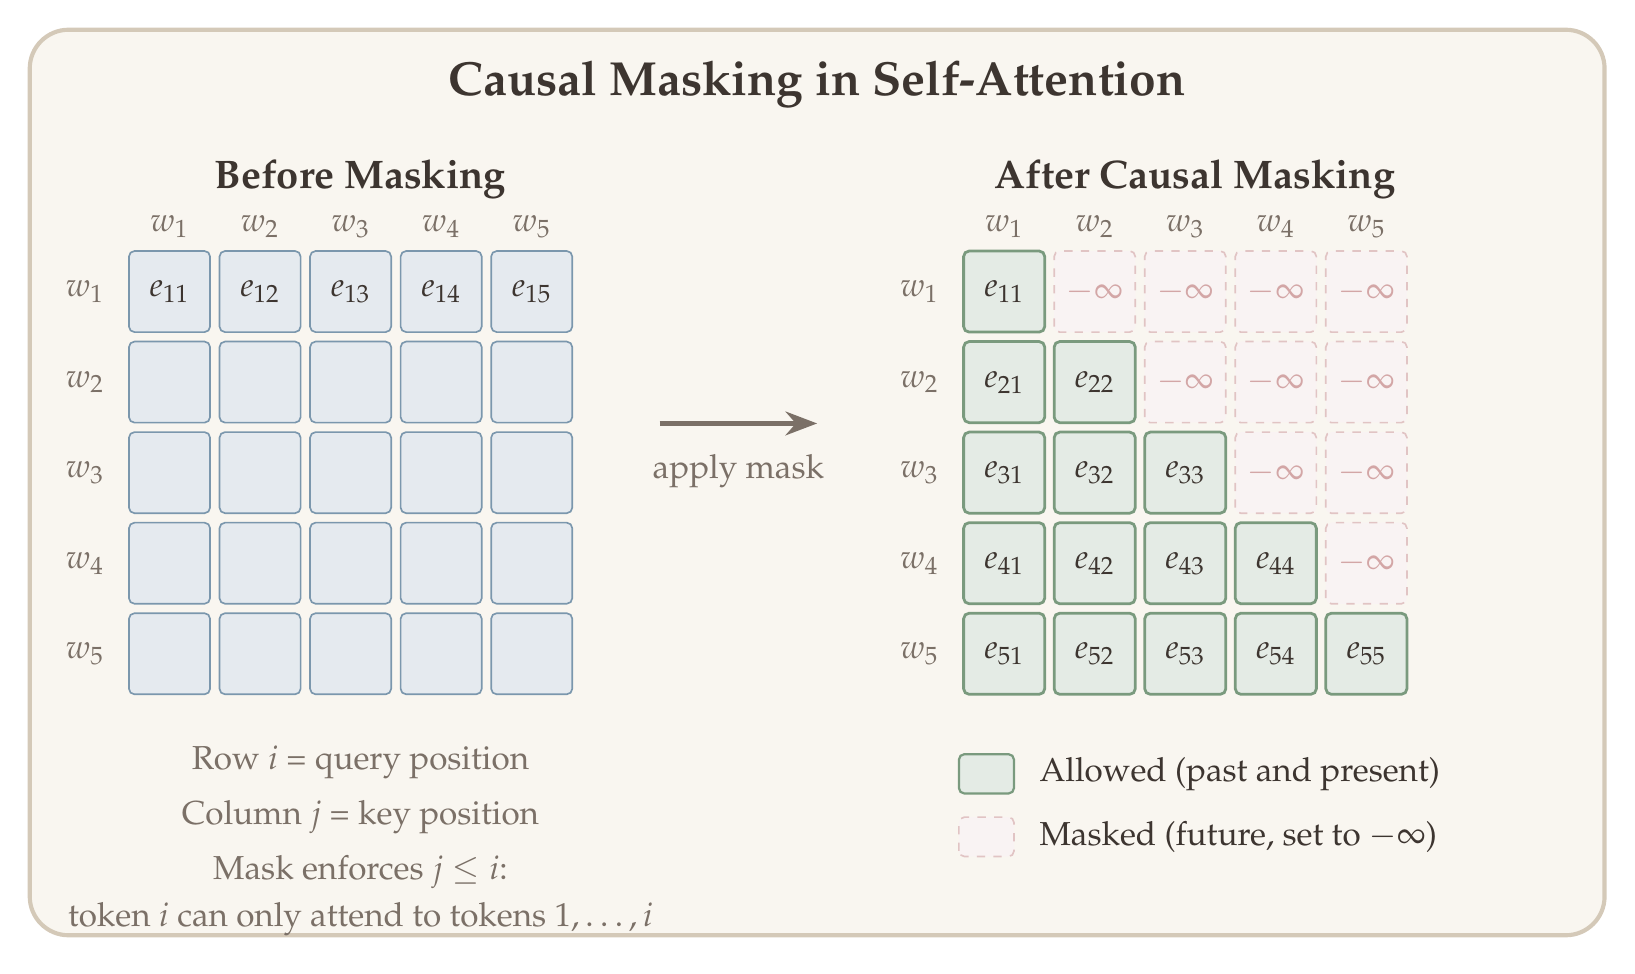
\begin{tikzpicture}[
  >={Stealth[length=4mm, width=3mm]},
  every node/.style={text=dkbrown, font=\large},
]

% Background
\fill[cream, rounded corners=14pt] (0,0) rectangle (20,11.5);
\draw[border, line width=1.5pt, rounded corners=14pt] (0,0) rectangle (20,11.5);

% Title
\node[font=\LARGE\bfseries, text=dkbrown] at (10,10.8) {Causal Masking in Self-Attention};

% ============ Left: Before Masking ============
\node[font=\Large\bfseries] at (4.2,9.6) {Before Masking};

% Grid parameters
\def\cellsize{1.15}
\def\lx{1.2}  % left grid x start
\def\ly{3.0}  % left grid y start (bottom-left of grid)

% Row labels
\foreach \i/\lab in {0/$w_1$, 1/$w_2$, 2/$w_3$, 3/$w_4$, 4/$w_5$} {
  \node[font=\large, text=wmgray] at ({\lx - 0.5}, {\ly + 4*\cellsize - \i*\cellsize + \cellsize/2}) {\lab};
}
% Column labels
\foreach \j/\lab in {0/$w_1$, 1/$w_2$, 2/$w_3$, 3/$w_4$, 4/$w_5$} {
  \node[font=\large, text=wmgray] at ({\lx + \j*\cellsize + \cellsize/2}, {\ly + 5*\cellsize + 0.25}) {\lab};
}

% All cells filled (unmasked)
\foreach \i in {0,...,4} {
  \foreach \j in {0,...,4} {
    \fill[stblue!20, rounded corners=2pt]
      ({\lx + \j*\cellsize + 0.06}, {\ly + (4-\i)*\cellsize + 0.06})
      rectangle ({\lx + (\j+1)*\cellsize - 0.06}, {\ly + (5-\i)*\cellsize - 0.06});
    \draw[stblue, line width=0.6pt, rounded corners=2pt]
      ({\lx + \j*\cellsize + 0.06}, {\ly + (4-\i)*\cellsize + 0.06})
      rectangle ({\lx + (\j+1)*\cellsize - 0.06}, {\ly + (5-\i)*\cellsize - 0.06});
  }
}

% Score labels (first row only for clarity)
\foreach \j/\lab in {0/$e_{11}$, 1/$e_{12}$, 2/$e_{13}$, 3/$e_{14}$, 4/$e_{15}$} {
  \node[font=\large] at ({\lx + \j*\cellsize + \cellsize/2}, {\ly + 4*\cellsize + \cellsize/2}) {\lab};
}

% ============ Arrow in the middle ============
\draw[wmgray, line width=2pt, ->] (8.0,6.5) -- (10.0,6.5);
\node[font=\large, text=wmgray] at (9.0,5.9) {apply mask};

% ============ Right: After Causal Masking ============
\node[font=\Large\bfseries] at (14.8,9.6) {After Causal Masking};

\def\rx{11.8}  % right grid x start

% Row labels
\foreach \i/\lab in {0/$w_1$, 1/$w_2$, 2/$w_3$, 3/$w_4$, 4/$w_5$} {
  \node[font=\large, text=wmgray] at ({\rx - 0.5}, {\ly + 4*\cellsize - \i*\cellsize + \cellsize/2}) {\lab};
}
% Column labels
\foreach \j/\lab in {0/$w_1$, 1/$w_2$, 2/$w_3$, 3/$w_4$, 4/$w_5$} {
  \node[font=\large, text=wmgray] at ({\rx + \j*\cellsize + \cellsize/2}, {\ly + 5*\cellsize + 0.25}) {\lab};
}

% Allowed cells (lower triangle j <= i)
\foreach \i in {0,...,4} {
  \foreach \j in {0,...,4} {
    \pgfmathparse{int(\j <= \i)}
    \ifnum\pgfmathresult=1
      % Allowed cell
      \fill[sage!20, rounded corners=2pt]
        ({\rx + \j*\cellsize + 0.06}, {\ly + (4-\i)*\cellsize + 0.06})
        rectangle ({\rx + (\j+1)*\cellsize - 0.06}, {\ly + (5-\i)*\cellsize - 0.06});
      \draw[sage, line width=1pt, rounded corners=2pt]
        ({\rx + \j*\cellsize + 0.06}, {\ly + (4-\i)*\cellsize + 0.06})
        rectangle ({\rx + (\j+1)*\cellsize - 0.06}, {\ly + (5-\i)*\cellsize - 0.06});
      \pgfmathtruncatemacro{\ii}{\i+1}
      \pgfmathtruncatemacro{\jj}{\j+1}
      \node[font=\large] at ({\rx + \j*\cellsize + \cellsize/2}, {\ly + (4-\i)*\cellsize + \cellsize/2})
        {$e_{\ii\jj}$};
    \else
      % Masked cell
      \fill[rosefade!8, rounded corners=2pt]
        ({\rx + \j*\cellsize + 0.06}, {\ly + (4-\i)*\cellsize + 0.06})
        rectangle ({\rx + (\j+1)*\cellsize - 0.06}, {\ly + (5-\i)*\cellsize - 0.06});
      \draw[rosefade!40, line width=0.6pt, rounded corners=2pt, dashed]
        ({\rx + \j*\cellsize + 0.06}, {\ly + (4-\i)*\cellsize + 0.06})
        rectangle ({\rx + (\j+1)*\cellsize - 0.06}, {\ly + (5-\i)*\cellsize - 0.06});
      \node[font=\large, text=rosefade!60] at ({\rx + \j*\cellsize + \cellsize/2}, {\ly + (4-\i)*\cellsize + \cellsize/2})
        {$-\infty$};
    \fi
  }
}

% Legend
\fill[sage!20, rounded corners=2pt] (11.8,1.8) rectangle (12.5,2.3);
\draw[sage, line width=0.8pt, rounded corners=2pt] (11.8,1.8) rectangle (12.5,2.3);
\node[font=\large, anchor=west] at (12.7,2.05) {Allowed (past and present)};

\fill[rosefade!8, rounded corners=2pt] (11.8,1.0) rectangle (12.5,1.5);
\draw[rosefade!40, line width=0.6pt, dashed, rounded corners=2pt] (11.8,1.0) rectangle (12.5,1.5);
\node[font=\large, anchor=west] at (12.7,1.25) {Masked (future, set to $-\infty$)};

% Left annotation
\node[font=\large, text=wmgray] at (4.2,2.2) {Row $i$ = query position};
\node[font=\large, text=wmgray] at (4.2,1.5) {Column $j$ = key position};
\node[font=\large, text=wmgray] at (4.2,0.8) {Mask enforces $j \leq i$:};
\node[font=\large, text=wmgray] at (4.2,0.2) {token $i$ can only attend to tokens $1, \ldots, i$};

\end{tikzpicture}
\end{document}
